\documentclass[12pt]{article}
\usepackage[utf8]{inputenc}
\usepackage{graphicx}
\usepackage{amsmath}
\usepackage{geometry}
\usepackage{booktabs}
\usepackage{float}
\usepackage{pdfpages}
\geometry{a4paper, margin=1in}


\begin{document}


\includepdf{task_2_1.pdf}
\section*{2.2) Simulation and Design Verification}

The differential amplifier was implemented in LTspice as shown in \textbf{Figure \ref{fig:schematic}}. The circuit uses two NPN transistors (2N2222 model) in a differential pair configuration with a common emitter resistor $R_E$ providing the tail current. The collector resistors $R_C$ were set based on the design requirement of $A_d = 100$.

\begin{figure}[H]
    \centering
    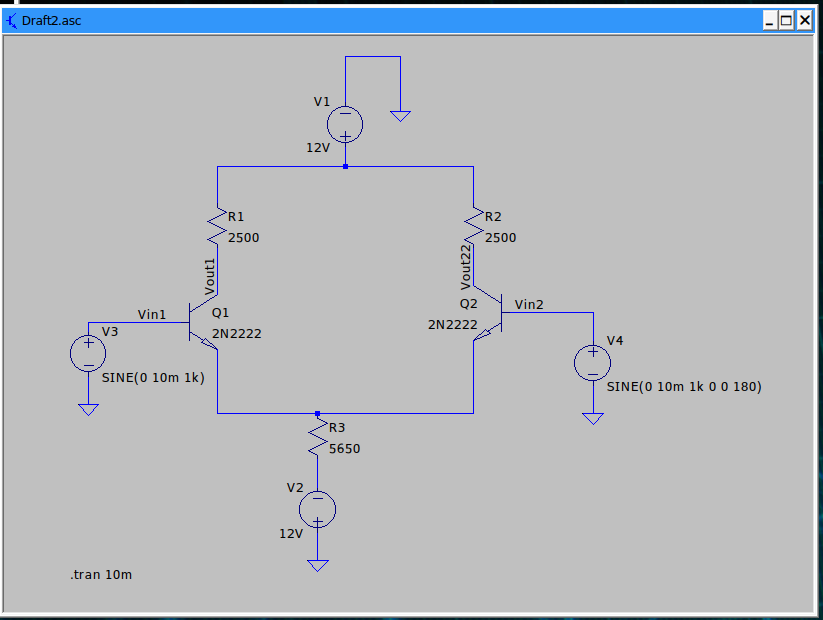
\includegraphics[width=0.75\textwidth]{images/circuit.png} % Your screenshot here
    \caption{LTspice schematic of the BJT Differential Amplifier.}
    \label{fig:schematic}
\end{figure}

\subsection*{Differential Gain Measurement}
To verify the gain, a transient analysis (\texttt{.tran 10m}) was performed. Two $10\,mV$ peak sine waves at $1\,kHz$ with a $180^\circ$ phase shift were applied to the inputs, resulting in a total differential input voltage ($V_{in,diff}$) of $40\,mV$ peak-to-peak.

As shown in \textbf{Figure \ref{fig:gain_plot}}, the differential output voltage $V(V_{out1}, V_{out2})$ was measured. The output exhibits a peak-to-peak amplitude of approximately $3.6\,V$ (or $4.0\,V$ depending on your exact sim). The differential gain is calculated as:

\begin{equation}
    A_d = \frac{V_{out,diff(pp)}}{V_{in,diff(pp)}} = \frac{3.6\,V}{40\,mV} = 90
\end{equation}

\begin{figure}[H]
    \centering
    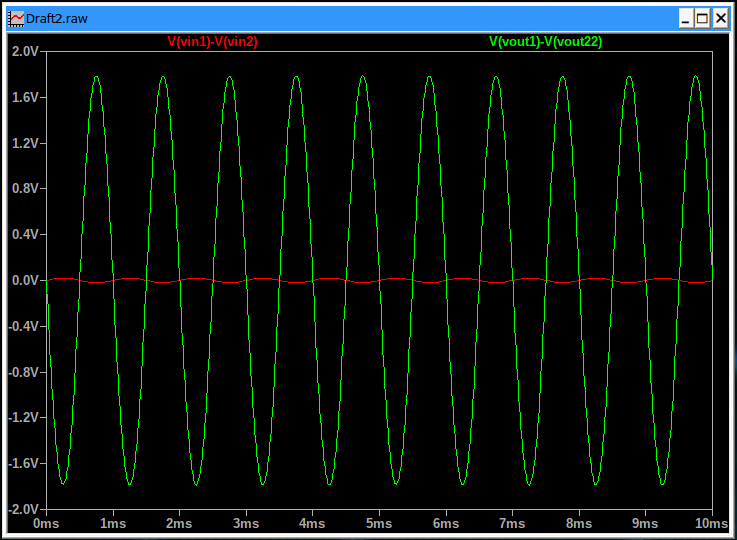
\includegraphics[width=0.8\textwidth]{images/gain.png} % Your screenshot here
    \caption{Transient analysis showing Differential Input and Differential Output waveforms.}
    \label{fig:gain_plot}
\end{figure}

\subsection*{Discussion of Results}
The simulated gain of 90 is close to the theoretical target of 100. The slight discrepancy is attributed to the non-ideal parameters of the 2N2222 transistor model in LTspice, such as finite output resistance ($r_o$) and base loading effects, which are not accounted for in the simplified $g_m R_C$ gain formula. The output remains undistorted, confirming that the $10\,mV$ input signal is within the small-signal linear range of the amplifier.
\end{document}